% Chapter 2

\chapter{TAXII} % Main chapter title

\label{Chapter2} % For referencing the chapter elsewhere, use \ref{Chapter1} 

\lhead{\til}
\rhead{\fu}
\lfoot{Chapter 2. \emph{TAXII}} % This is for the header on each page - perhaps a shortened title

%----------------------------------------------------------------------------------------

\section{Background}

El intercambio de información se ha tornado critico contra los adversarios actuales.
Actualmente un número creciente de organizaciones comparten 
información de amenazas con el fin de tener un visión más amplia de las 
actividades de los adversarios y así ayudar a administrar los recursos de las 
organizaciones para obtener el mejor resultado posible de sus defensas. 
La capacidad de compartir información de forma automática con un gran número
de comunidades y que dicha información sea completa no existe en la actualidad. 
El objetivo que plantea TAXII es extender 
la capacidad de compartir indicadores permitiendo intercambios robustos, seguros 
y de gran volumen de datos los cuales deben poseer información mas expresiva de 
amenazas informáticas.

TAXII es un conjunto de especificaciones técnicas y de documentación para 
permitir el intercambio de información procesable entre organizaciones. Para 
ello se definen protocolos y formatos de datos para intercambiar información de 
forma segura la cual ayude a detectar, prevenir y mitigar amenazas informáticas 
en tiempo real. No se buscan definir acuerdos para el intercambio de 
información, gobierno o aspectos técnicos del intercambio de información. En su 
lugar, permite a las organizaciones alcanzar una mejora en su situación respecto 
a las nuevas amenazas y además compartir información que ellos elijan con quien 
elijan de forma simple y rápida aprovechando las relaciones y sistemas 
existentes.

En el desarrollo de TAXII se busco consenso y participación de la comunidad. 
TAXII permite intercambio de información sobre amenazas de forma eficiente y 
comprensiva por medio de \emph{automatización} y \emph{articulación} de un 
modelo detallado de información. Para lograr esto, se utiliza una representación 
estándar de información de amenazas y un framework para soportar el intercambio 
de datos. El modelo permite el envío y recepción de un conjunto amplio de 
información de seguridad para soportar un amplio número de necesidades 
referentes al intercambio de información.

TAXII cubre un amplio número de casos de uso, tecnologías, especificaciones e 
implementaciones. Los casos de uso son desarrollados de manera secuencial, 
permitiendo un conjunto inicial de casos de usos que permite el intercambio e 
información. TAXII utiliza protocolos y especificaciones existentes siempre que 
es posible y se integra con mecanismos de intercambio de información existentes 
para reducir los costos de implementación y permitir la adopción rápida por 
parte de organizaciones ya establecidas que ya intercambian información.

\subsection{Fundamentos}
Las estrategias de defensa se deben adaptar al creciente número, frecuencia y 
complejidad de los ataques que se llevan a cabo. Actualmente la estrategia 
predominante se refiere a bloquear los ataques y arreglar las vulnerabilidades, 
esta estrategia se basa en alertas. Si bien puede ser efectiva contra algunas 
amenazas no logra detener ataques avanzados o proveer información sobre las 
actividades de un atacante luego de que la red fue penetrada. Una estrategia más 
adecuada es \emph{``cyber kill-chain''} la cual se representa a continuación.

La estrategia presentada busca descomponer las fases de un ataque con la 
finalidad de obtener una amplia comprensión del ataque y el atacante así como 
mejorar las posibilidades de defensa.

\begin{center}
    \begin{tabular}{ | l | p{8cm} |}
    \hline
    Fase de la cadena & Descripción \\ \hline
    Reconocimiento & El adversario identifica e investiga los objetivos. \\ \hline
    Armado & El conjunto de herramientas de ataque son empaquetadas para entrega
     y ejecución en la computadora o red de la víctima.  \\ \hline
    Entrega & La herramienta o herramientas empaquetadas son entregadas en el objetivo. \\ \hline
    Explotación & Se ejecuta el ataque inicial en el objetivo.  \\ \hline
    Control & El adversario comienza a dirigir los sistemas de la víctima para realizar acciones. \\ \hline 
    Ejecución & El adversario comienza a realizar los requerimientos de su misión.  \\ \hline
    Mantenimiento & Se logra un acceso a largo plazo.  \\ \hline
    \end{tabular}
\end{center}

Los primeros pasos de esta estrategia representan una oportunidad para detectar 
y mitigar las amenazas de forma proactiva antes de que el adversario realice un 
acceso no autorizado en los sistemas de la organización. En los pasos 
posteriores es donde se realiza la detección, respuesta y aseguramiento de los 
activos más importantes. Al entender al adversario los defensores tienen una 
mejor oportunidad para descubrir y responder al ataque. Actualmente se busca que 
las defensas anticipen y mitiguen las amenazas antes de que sean mas difíciles 
de encontrar y erradicar utilizando los métodos tradicionales de detección y 
respuesta.

Para poder realizar esto es necesario que se realice una actividad de cyber inteligencia,
recolecte información referente a ataques, con esta información analistas pueden 
agrupar patrones de actividades similares, atribuir actividades a ciertos actores, 
identificar e implementar estrategias de mitigación de forma rápida y anticiparse al 
lanzamiento de ataques similares en el futuro.

Para aprovechar de forma más adecuada los beneficios de la cyber inteligencia, 
las organizaciones deben compartir la información recolectada (incluyendo las 
estrategias de defensa entre otras) con socios de su confianza. De esta forma se 
obtiene una imagen mas completa de las actividades del adversario y de las 
acciones defensivas que se deben realizar. [1] Por medio del análisis del 
comportamiento de los adversarios en distintos objetivos y en un periodo de 
tiempo, los defensores son capaces de identificar un conjunto importante de 
indicadores y tácticas, técnicas y procedimientos (TTPs). De esta forma se 
obtiene información de los objetivos y las estrategias lo cual permite al 
defensor predecir el comportamiento del ataque y generar defensas dinámicas.

\subsection{Comunidades}
Hoy en día un número creciente de organizaciones buscan compartir información de 
las amenazas. Con esto ha crecido el número y tipo de las comunidades que buscan 
compartir información. Se pueden encontrar tres tipos de comunidades:
\begin{itemize}
  \item Peer
  \item Comerciales
  \item Gobierno
\end{itemize}

La necesidad primordial entre dichas organizaciones es la confianza dado que 
compartir información sensible podría exponer a una organización a un daño en su 
reputación, demandas o advertir a un adversario con lo cual el trabajo realizado 
fuera inútil. Se deben definir medidas para la protección de los datos como 
restricciones en el manejo de los datos, sanitización de los datos y el 
establecimiento de confianza entre las dos partes. Esto es particularmente 
importante cuando las organizaciones forman parte de varias comunidades para el 
intercambio de amenazas de seguridad. Se puede ver que lo que es compartido con 
una comunidad no necesariamente debería ser compartido con otra.
Las comunidades entre peers son las más comunes, en estas organizaciones o 
individuos con un propósito común se unen para mejorar las defensas colectivas 
contra adversarios comunes o conjuntos de adversarios.

Las comunidades comerciales se basan en membresias por parte de los miembros y 
son altamente anónimas. La organización comercial maneja de forma centralizada 
la información y la distribuye entre los miembros de la organización. Estas 
organizaciones proveen una forma rápida de obtener información, además puede ser 
más amplia que la información especializada que es compartida por pares y puede 
que no siempre sea aplicable a las necesidades de una organización.

Las comunidades gubernamentales  son establecidas y manejadas por el gobierno, 
son voluntarias u obligatorias e incluyen participantes tanto del gobierno como 
de la industria privada. En ellas el gobierno controla la información y la 
diseminación de esta, cabe señalar que así como en las comunidades comerciales 
la información y los participantes son altamente confidenciales.
\subsection{Modelos} %Ver titulo
Hay tres modelos principales para el intercambio de información entre 
organizaciones:
\begin{itemize}
  \item hub and spoke
  \item peer to peer
  \item source/subscriber
\end{itemize}
En el método hub and spoke, una entidad controla la recepción y la diseminación 
de los datos. La entidad hub usualmente anonimiza los datos 
recolectado de las amenazas y provee una análisis adicional a los participantes. 
Este modelo es comúnmente visto en comunidades de gobierno o comerciales.
En el modelo peer to peer, los participantes intercambian y reciben información 
directamente de los otros participantes. La información es compartida entre 
todos los miembros de la comunidad por igual y la fuente esta claramente 
identificada.

El modelo faltante es el de source/suscriber, este modelo es utilizado por las 
comunidades comerciales que proveen de información. El proveedor de información 
envía regularmente información a todos los suscriptores y estos podrían 
eventualmente enviarle información a la fuente. Usualmente, en este modelo la 
información esta codificada de una manera propietaria y puede faltar 
información esencial sobre algunas intentos de irrupción. Presenta la ventaja de 
que se tiene acceso rápido a un conjunto de datos amplio y es útil para 
organizaciones con recursos limitados.

\subsection{Métodos para el intercambio de información}

Hay múltiples métodos para el intercambio de información. Usualmente, el método 
juega un rol significante en los tipos, volúmenes y naturaleza de la información 
compartida con la comunidad. Algunos medios de intercambio limitan el tipo de 
contenido que es compartido de forma sencilla mientras que otros promueven 
ciertos tipos de intercambio.
Algunos métodos comunes son:
\begin{itemize}
  \item Email lista de servidores
  \item Foros de discusión
  \item wikis
  \item repositorios de datos
\end{itemize}
La mayoría de estos métodos no permiten el consumo de información de amenazas de 
forma automática. La mayoría de los consumidores rutinariamente toman esta 
información y la sintetizan en sus bases de datos locales.
Existen varios esfuerzos para generar arquitecturas abiertas, estándar 
basados en indicadores e información de incidentes. La realidad es que ninguno 
de estos a podido convertirse en un estándar para el intercambio entre comunidades.


\subsection{Información compartida}
Actualmente los indicadores que se comparten son sistemas maliciosos, actividades de red 
o cyber observables de interes como las direcciones de IP, nombres de dominio, 
nombres de archivos o direcciones de email. En algunos casos, la información 
compartida esta enfocada en una amenaza en particular, como las botnets. En 
otros casos se incluye malware en uso u otros TTP. La información compartida 
esta establecida generalmente por la comunidad o por el grado de confianza entre 
las partes.

\subsubsection{Limitaciones}

Compartir información ha ayudado a mejorar las capacidades defensivas de 
numerosas organizaciones. Sin embargo, las aproximaciones actuales no han 
logrado que se llegue al máximo potencial. Los procesos para compartir 
información son manuales, llevan mucho tiempo, son repetitivos y en muchos casos 
requieren que  las organizaciones re escriban o traduzcan la información a una 
amplia variedad de formatos. La información es además compartida por medios 
inseguros. Debido a la variedad de formatos y los protocolos en uso, así como 
los procesos manuales involucrados, esta técnica se lleva a cabo entre pocas 
organizaciones en las que se confía.


Otro factor que hace que sea ineficiente el intercambio de información, menos escalable y que consuma mucho tiempo es el uso de tecnologías 
y/o formatos propietarios, presentandose la necesidad de desarrollar un amplio 
número de scripts y módulos para permitir compartir información por fuera de las 
comunidades. Para aquellas comunidades con algún grado de automatización, sus 
modelos son generalmente bajos en prestaciones y usan soluciones propietarias,
comerciales o adaptadas a su comunidad.

Otra limitación se presenta en la naturaleza atómica de la mayoría de los 
indicadores. Por ejemplo, cuando una IP en particular es identificada como 
sospechosa el esfuerzo que debe realizar el adversario para cambiar la IP es 
prácticamente cero. Confiar únicamente en indicadores atómicos sin contexto 
puede proveer un gran número de falsos positivos llevando a un desperdicio en 
tiempo de análisis.

\subsubsection{Motivación}

Una mejor solución para compartir información es necesaria, una que sea 
utilizada por diferentes comunidades y modelos para compartir información, 
permitiendo diferentes métodos para compartir, y que soporte un rango amplio de 
datos. En particular, los objetivos de la solución ideal son:
\begin{itemize}
  \item Permite compartir información de forma más rápida y precisa
  \item Reducir el análisis humano y liberar a los recursos humanos para 
  realizar trabajo de análisis más valioso.
  \item Mover las amenazas más conocidas para que sean analizadas por 
  computadoras.
  \item Permitir que se comparta de forma automática un gran rango de datos, 
  siendo estos datos complejos y no los simples, atómicos indicadores. Esto 
  debería permitir una defensa activa.
  \item Proteger la información intercambiada.
  \item Permitir que se agregue información a las bases locales con información de contexto y 
  discreción, limitando el número de analistas que acceden a la información.
  \item Permitir la colaboración de analistas de distintas organizaciones en los 
  incidentes que sean un reto.
  \end{itemize}
  
 \subsection{Que es TAXII}
 TAXII es un conjunto de especificaciones técnicas y documentación para el 
 intercambio de información de alta fidelidad, dicho intercambio es 
 independiente de la plataforma y realizado de forma segura. Esta diseñado de 
 forma que permita la interoperabilidad de diferentes soluciones en lugar de 
 ligarse a una tecnología o producto en particular. Además se busca incentivar a 
 los proveedores de tecnología a incorporar soporte para las especificaciones de 
 TAXII en sus productos.
 
 Ha sido desarrollado con consenso y participación de la comunidad, con la 
 finalidad de permitir un intercambio eficiente y comprensivo de la 
 información detallada, de forma automática y articulada. Para lograr esto, 
 TAXII utiliza una representación estándar de la información y define un 
 framework para soportar el intercambio. TAXII ofrece una forma de describir e 
 intercambiar los indicadores, dejando a los proveedores la libertad de 
 determinar como sus productos producen, consumen o toman ventaja de los flujos 
 de información especificados por TAXII.
 
\begin{figure}[ht!]
  \centering
    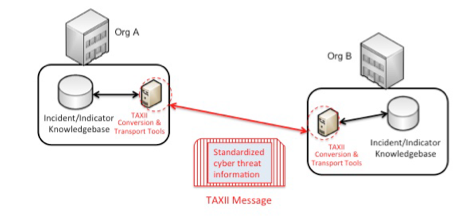
\includegraphics[width=150mm]{./Figures/TAXIIArchitecture1.png}
\end{figure}

 
 \subsection{Objetivos de TAXII}
 Los objetivos de TAXII son:
 \begin{itemize}
   \item Permitir el intercambio seguro y rápido de información referente a 
   amenazas entre comunidades de defensores de seguridad.
   \item Lograr un estándares para permitir compartir indicadores entre otros 
   elementos entre organizaciones.
   \item Extender el intercambio de indicadores para permitir intercambios 
   seguros, robustos y de gran volumen que tengan una expresividad mayor a la 
   actual.
   \item Soportar un amplio número de casos de uso y practicas comunes a las 
   comunidades.
   \item Tomar los estándares existentes que sean adecuados.
   \item Llegar a una adopción por parte de organizaciones internacionales de 
   estándares.
 \end{itemize}
 
 TAXII no ha creado una comunidad para compartir, sino que permite que las 
 comunidades compartan. TAXII mejora las deficiencias existentes proveyendo 
 especificaciones abiertas y comunes para transportar los mensajes con 
 información con capacidades como encriptación, autenticación, 
 direccionamiento, alertas y pedidos entre sistemas.
  
  \subsection{Representación estándar de la información}
TAXII utiliza el lenguaje STIX para representar la información. STIX es un 
lenguaje desarrollado por la comunidad para la especificación, captura, 
caracterización y comunicación de información de amenazas cibernéticas de forma 
estandarizada. STIX provee una arquitecutra unificada que soporta varios tipos 
de información entre los cuales se incluyen Cyber Observables, Indicadores, 
Incidentes, tácticas, técnicas y procedimientos de los adversarios, etc.

Para maximizar la compatibilidad y facilidad de adopción, STIX utiliza varios 
standards como CybOX, Common vulnerabilities and exposures (CVE) y common 
platform enumeration (CPE).

\subsection{Un framework de Intercambio}
La segunda parte necesaria para automatizar el intercambio de información es 
especificar como esta es compartida. Para alcanzar esto, TAXII define 
especificaciones técnicas y documentación de soporte. En particular, las 
especificaciones de TAXII definen un conjunto de capacidades necesarias para el 
transporte exitoso de mensajes, o como los mensajes TAXII llegan del punto A al 
B. Los mensajes TAXII llevan datos de amenazas informáticas transformadas a 
formato STIX. El conjunto completo de los mensajes incluye mensajes con datos y 
de control.

TAXII utiliza protocolos y especificaciones existentes siempre que sea posible y 
los integra con los mecanismos actuales para reducir los costos de 
implementación y permitir una adopción rápida por parte de las organizaciones ya 
establecidas que ya comparten información. TAXII esta siendo desarrollado de 
forma modular para soportar una variedad de mecanismos y formatos de datos para 
ser intercambiados.

\subsection{Casos de Uso}
TAXII ha sido desarrollado para soportar casos de uso comunes para el 
intercambio de información.

Alertas o Advertencias públicas

Estas son advertencias al publico en general o a varios asistentes de varios 
CSIRT, enviadas a todos los suscriptores.
Estas alertas son de una naturaleza tan amplia que no necesitas ser encriptadas 
o no se necesitan autorizaciones. Sin embargo es importante una firma digital  
para asegurar la autenticidad. Las entidades u organizaciones deben ser 
especificadas para identificar la fuente de la alerta.

Alertas y Reportes privados

Las alertas privadas son similares a las públicas, exceptuando que la 
información compartida es sensible y restringida a los socios que comparten 
datos. Los mecanismos para enviar datos deberían ser similares a los de las 
alertas públicas. Como las alertas y reportes se suponen sensibles y no para el 
uso general, es importante que TAXII soporte formas adecuadas de encriptación, 
autenticación, autorización e identificación de datos. Dependiendo en la 
naturaleza de las comunicaciones, manejo explícito de marcas o restricciones 
en datos compartidos debería ser necesario.

Las alertas son generalmente cortas, mensajes estándares con indicadores muy 
específicos o acciones especificadas.

Los reportes son mensajes mas largos, y pueden incluir reportes de incidentes, 
análisis de malware, análisis de amenazas u otras observaciones.

Soportes para Queries

Es común que los analistas de amenazas busquen información de otros entre sus comunidades
así como por fuera de ellas.
\begin{itemize}
  \item RFI (Request for Information): es un mensaje simple que se espera sea 
  manejado de forma manual y que permite que se pida información.
  \item Repository Search: Para este tipo de query, es esperado que una 
  organización ofrezca repositorios en los que buscar, los cuales podrían ser 
  compatibles con TAXII o STIX.
\end{itemize}

\subsubsection{Transferencia}

Varias organizaciones que transfieren información necesitan en algunas 
instancias agregar miembros. El nuevo miembro necesitas obtener los datos del 
repositorio de la organización. Por ello se desea un caso de uso para realizar 
el intercambio de un gran volúmen de datos.

\section{Componentes de TAXII}
\begin{itemize}
  \item Especificación de TAXII: Define la especificación de los componentes y 
  provee guía y requerimientos sobre como dichas especificaciones interoperan en 
  TAXII.
  \item Especificación de servicios de TAXII: Define una serie de servicios que 
  deben ser implementados para ser compatible con TAXII. Describe información 
  intercambiada a un nivel alto y no se limita a ningún mecanismo de 
  intercambio en especial.
  \item Implementación de Servicios: Se realiza una implementación de los 
  servicios TAXII para un mecanismo de intercambio. Cada implementación de 
  servicios provee guía técnica y requerimientos para implementar la 
  especificación de los mecanismos de intercambio.
  \item Modelo de datos de mensajes: Se define una estructura para los mensajes 
  TAXII, incluyendo header, payload, control y mensajes de datos. Los mensajes 
  de datos utilizan STIX para el payload de los mensajes TAXII.
  \item Implementaciones de los mensajes de datos: Es una implementación del 
  modelo de datos de mensajes, incluyendo el payload STIX.
   Cada implementación de mensajes define la guía técnica y 
  requerimientos  para utilizar un formato de mensajes particular para expresar 
  el modelo de datos de mensajes.
\end{itemize}

\subsection{TAXII Toolkit}
Es provisto para soportar la adopción de TAXII y asistir en el desarrollo de 
capacidades compatibles. El toolkit provee una colección de implementaciones de 
referencia, un conjunto de herramientas y una colección de librerías e 
interfaces.

\Section{Especificaciones de TAXII}

TAXII esta definido por múltiples especificaciones relacionadas. Esta sección 
describe las especificaciones definidas en TAXII.

\begin{itemize}
  
\item Especificación de Servicios (Service Specification): Provee los requerimientos por los cuales se definen los servicios e intercambios 
de TAXII. No provee detalles respecto al formato de los datos o como los 
mensajes TAXII son transportados por la red. Dichos detalles y requerimientos 
pueden ser encontrados en Protocol Binding Specification y Message Binding 
Specification.
\item Especificación de protocolos de enlace (Protocol Binding Specification): 
Define los requerimientos para transportar mensajes TAXII por la red. Puede 
haber varias especificaciones creadas para TAXII. Cada especificación define 
requerimientos para transportar mensajes TAXII usando protocolos de red y se 
proveen requerimientos respecto a como los servicios TAXII son soportados por 
los protocolos de red.
\item Especificación de Mensajes (Message Binding Specification): Se definen 
requerimientos para representar mensajes TAXII en un formato particular. Puede 
haber múltiples especificaciones para dichos mensajes. Se provee información 
detallada sobre como la información definida en la especificación de servicios 
es expresada en los mensajes.
\end{itemize}

\begin{figure}[ht!]
  \centering
    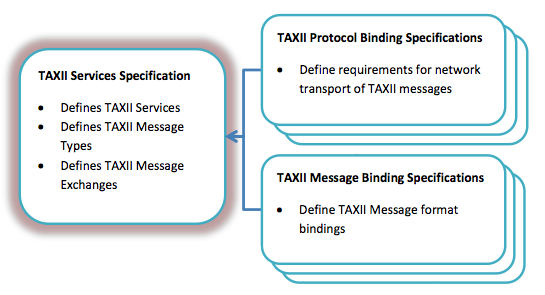
\includegraphics[width=150mm]{./Figures/TAXIIEspecification.png}
\end{figure}


Separación de la especificación de servicios, los protocolos de enlace y los 
mensajes existe para dar flexibilidad mientras TAXII evoluciona. Debido a que 
las organizaciones generalmente tienen restricciones respecto a los protocolos 
que soportan, TAXII busca no ligarse a un único protocolo que excluya a una 
parte de la comunidad. Cuando se ve que la comunidad expresa interés en un nuevo 
protocolo o tipo de mensaje, TAXII puede dar soporte para ellos sin cambiar los 
componentes centrales.

Dos grupos que usen el mismo protocolo de red y formato de mensajes serán 
capaces de intercambios de información estructurada de forma automática. Las 
políticas de intercambio de los participantes puede limitar estos intercambios 
si es necesario, pero el uso de servicios compatibles con TAXII asegura que 
se puede intercambiar cualquier información con los mecanismos definidos por 
TAXII. Los grupos que usen diferentes protocolos o formatos de mensajes no serán 
capaces de comunicarse directamente, pero como están utilizando mensajes y 
servicios en el núcleo de las comunicaciones de sus comunidades significa que es 
posible establecer caminos para que ocurra la interacción.

\subsection{Especificación de Servicios}
Esta especificación provee normativas respecto a los servicios, mensajes e 
intercambio de mensajes en TAXII. No provee detalles respecto a como los 
mensajes son transportados, dejando eso a la especificación de los protocolos de 
enlace. Si bien se provee información relacionada a la información presente en 
los mensajes TAXII, no da información respecto a como los mensajes TAXII son 
expresados.


\subsubsection{Unidades funcionales de TAXII}


Las unidades funcionales de TAXII representan conjuntos discretos de actividades 
requeridas para soportar TAXII. Una unidad funcional representa algún componente 
con un rol bien definido en TAXII.

\begin{itemize}
  \item TAXII Transfer Agent (TTA) : Es una unidad funcional conectada a la red 
  que envía o recibe mensajes TAXII. Una TTA interactúa con otras TTAs por medio 
  de la red y maneja los detalles de los requerimientos del protocolo de uno o 
  más TAXII Protocol Binding Specifications. Una TTA provee mensajes TAXII a un 
  TAXII Message Handler permitiendo que este último sea independiente del 
  protocolo de red utilizado. De la misma forma, el TTA puede ser independiente 
  del contenido de los mensajes TAXII, dejando el manejo de la información al 
  TAXII Message Handler.
  \item TAXII Message Handler (TMH): Es una unidad funcional que produce y 
  consume mensajes TAXII. El TMH es responsable de parsear y construir mensajes 
  con el formato especificado en uno o mas TAXII Message Binding Specifications. 
  Un TMH interactúa con un TTA, el cual maneja los detalles necesarios para 
  transmitir mensajes por la red. El Back-end TAXII interactúa con el TMH para 
  convertir su contenido en mensajes TAXII, y llevar a cabo actividades basadas 
  en los mensajes TAXII que son recibidos por el TMH.
  \item TAXII Back-end: Cubre todas las unidades funcionales distintas al TTA y 
  al TMH. Las especificaciones de TAXII no proveen requerimientos sobre como son 
  implementadas las capacidades en un back-end mas allá de como debe interactuar 
  con el TMH. Las organizaciones o implementadores pueden decidir que 
  capacidades implementar según los servicios TAXII que deseen soportar o según 
  como quieren dar ese soporte.
  \item Arquitectura TAXII: Cubre los aspectos de las unidades funcionales de la 
  infraestructura de productor o consumidor que prove o utiliza servicios TAXII. 
  Una arquitectura TAXII incluye una TTA, un TMH y un back-end TAXII.
  
  
\begin{figure}[ht!]
  \centering
    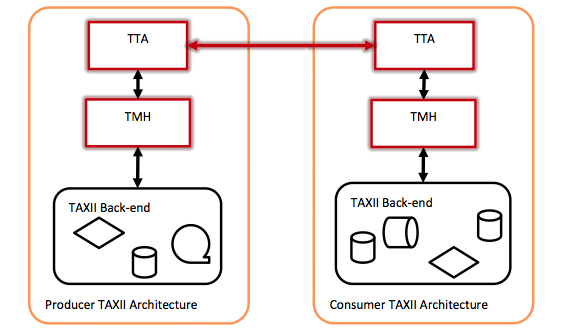
\includegraphics[width=150mm]{./Figures/TAXIIArchitecture.png}
\end{figure}
  
\end{itemize}

\subsubsection{Roles en TAXII}

Los roles en TAXII son utilizados de acuerdo al uso que se hace de los servicios 
especificados en TAXII.
\begin{itemize}
  \item Productor es el rol de una entidad que es la fuente de información 
  estructurada de amenazas.
  \item Consumidor es el rol de la entidad que recibe información estructurada 
  sobre amenazas.
\end{itemize}

\subsubsection{Componentes de red}

Los siguientes términos son utilizados para definir componentes de una 
implementación TAXII utilizando un modelo cliente-servidor.
\begin{itemize}
  \item Una implementación TAXII es un implementación específica de una 
  arquitectura TAXII.
  \item Servidor TAXII Es una implementación que provee uno o mas servicios 
  TAXII. Para soportar esta funcionalidad, se asume que un servidor TAXII esta 
  continuamente esperando tráfico de red.
  \item Cliente TAXII Es una implementación TAXII que inicia intercambio con un 
  servidor TAXII. Un cliente no necesita una conexión persistente con Internet 
  para operar pero puede abrir conexiones cuando desea interactuar con un 
  servidor y desconectarse de Internet cuando la conexión a terminado.
  \item TAXII endpoint denota una implementación TAXII que puede ser un servidor 
  o un cliente
\end{itemize}


\subsection{Capacidades}
La existencia de TAXII provee capacidades especificas para aquellos que desean 
compartir información de amenazas cibernéticas. Las capacidades TAXII son el 
nivel mas alto en el cual se pueden expresar las acciones de TAXII. Hay tres 
capacidades que soporta la actual versión de TAXII: push messaging, pull 
messaging y discovery.

\subsubsection{Push Messaging}

La información puede ser enviada de un productor a un consumidor. Esto puede 
reflejar una relación pre-existente entre el productor y el consumidor en la que 
el consumidor a pedido que se le envíen datos desde el productor. También puede 
usarse en caso de que el consumidor desee aceptar contribuciones de cualquier 
productor, y estos le envíen datos en cualquier momento.

\subsubsection{Pull Messaging}

Un consumidor puede requerir información de un productor. Esto no solo le 
permite al consumidor el control sobre el momento en el que recibe los datos 
sino que también le permite hacerlo sin tener que aceptar conexiones entrantes. 
Así como en push messaging, el productor y consumidos pueden tener acuerdos 
pre-existentes  para que el consumidor tenga acceso a los datos del productor. 
De forma alternativa, un productor puede hacer su información pública  y 
cualquer consumidor puede requerir sus datos.
La versión actual de pull messaging, limita a los consumidores a hacer pedidos 
por medio de las organizaciones productoras de los datos en lugar de por los 
datos en si. Todos los datos provistos por un productor deben estar organizados 
en grupos llamados "TAXII Data Feeds". Piezas individuales de información en un 
TAXII Data Feed son etiquetadas utilizando timestamps. El productor tiene total 
discresión sobre como el contenido se mapea en TAXII Data Feeds y en el 
significado de los timestamps. La capacidad de pull messaging esta atada a 
entender el contenido del productor.

\subsubsection{Discovery}

Para facilitar las comunicaciones automatizadas, TAXII soporta capacidades para 
descubrir los servicios específicos que ofrece un servidor o grupo de 
servidores, así como los protocolos o mensajes que este servidor ofrece. Esto no 
quita la necesidad del involucramiento humano para establecer acuerdos de 
cooperación lo cual esta por fuera del objetivo de TAXII. Sin embargo permite el 
intercambio de información respecto a las capacidades que un productor pudiera 
soportar y cuales son los mecanismos que utiliza para hacerlo.


\subsection{Servicios TAXII}
Los servicios TAXII representan un conjunto de mecanismos necesarios para 
soportar capacidades TAXII. Una implementación TAXII pudiera implementar alguno, 
todos o incluso ninguno de los servicios definidos.
TAXII define los siguientes servicios:
\begin{itemize}
  \item Servicio de descubrimiento: Es utilizado para recibir y responder a 
  mensajes que requieren información sobre los servicios ofrecidos.
  \item Feed Managment Service: Es utilizado para recibir o responder a mensajes 
  utilizados para el manejo de subscripciones a TAXII Data Feed.
  \item Inbox Service: Es utilizado para recibir información de amenazas 
  cibernéticas por medio de intercambios iniciados por el productor en intervalos 
  dictados por este.
  \item Poll Service: Es utilizado para recibir y responder a mensajes de pedido 
  a el TAXII Data Feed iniciados por el consumidor.
\end{itemize}

A continuación se describen los distintos servicios.

\subsubsection{Discovery Service}

Es un mecanismo para comunicar información referente al uso de servicios TAXII y 
a su disponibilidad. Para un pedido al servicio, se retorna una lista de los 
servicios TAXII y como estos pueden ser invocados. Un solo servicio de 
descubrimiento puede reportar servicios TAXII en diferentes equipos finales o 
incluso en múltiples organizaciones, los propietarios del servicio pueden 
definir su alcance a gusto. Un servicio de descubrimiento puede utilizar 
varios factores para determinar cuales servicios revelar ante una petición, 
incluyendo, pero no limitado a la entidad del cliente TAXII.
El servicio de descubrimiento debe soportar "Discovery Message Exchange".

\subsubsection{Feed Managment Service}

Es el mecanismo con el cual un consumidor pide información referente a TAXII 
Data Feeds, pidiendo subscripciones a estos, o modificando las existentes. Éste 
servicio facilita el intercambio de mensajes para manejar las subscripciones. 
No se entrega contenido de los TAXII Data Feed, en su lugar se envia 
contenido del TAXII Data Feed al servicio de Inbox de un consumidor en intercambios 
iniciados por un productor o en respuesta directa a un pedido del consumidor al 
servicio de poll.
Dicho servicio debe implementar soporte para subscription managment exchange.
Dicho servicio podría implementar soporte de feed information exchange.

\subsubsection{Inbox service}
Éste servicio es el mecanismo con el cual un consumidor acepta los mensajes en 
un intercambio iniciado por el productor. Un consumidor puede implementarlo 
para recibir datos del TAXII Data Feed.
El servicio de inbox debe implementar soporte para Data Push Exchange.

\subsubsection{Poll service}
Es provisto por un productor para permitir pedidos al TAXII Data Feed iniciados 
por  el consumidor. Un consumidor contacta a éste servicio explícitamente 
pidiendo el contenido del TAXII Data Feed. Los productores podrían ofrecer Data 
Feeds combinando envios al Inbox service del consumidor o por medio de pedidos 
al servicio de poll de productor.
Un implementación de éste servicio debe dar soporte a Data Poll Exchange.


\section{Intercambio mensajes TAXII}
Esta sección describe los mensajes de intercambio TAXII necesarios para soportar 
los servicios TAXII definidos antes. Estos intercambios solo consideran mensajes 
TAXII y son independientes a los protocolos sobre los cuales viajan los mensajes 
TAXII. En particular, esos protocolos podrían requerir intercambios de red 
adicionales antes de transmitir mensajes TAXII o romper un mensaje TAXII en 
multiples mensajes del protocolo subyacente que son transmitidos 
independientemente. Los siguientes diagramas representan conceptualmente la 
secuencia en la cual los mensajes TAXII son transmitidos y como actúan.

\subsection{Data Push Exchange}
En este intercambio, un mensaje STIX es transmitido desde un cliente a un 
servidor Inbox que este esperando. El mensaje STIX puede ser solicitado o no 
solicitado. El servidor inbox puede ser capaz de filtrar mensaje basandose en la 
autenticidad del emisor. Los mensajes enviados en este intercambio no deberian 
tener un campo 'In Response to' en su header.

\begin{figure}[ht!]
  \centering
    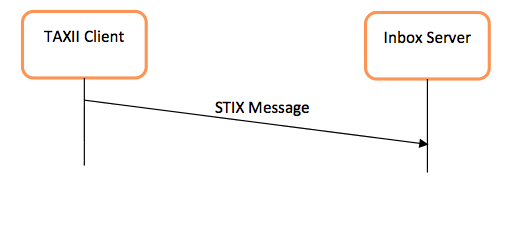
\includegraphics[width=150mm]{./Figures/DataPushExchange.png}
\end{figure}

El cliente TAXII envia un mensaje STIX al inbox server. El inbox server podria 
descartar el mensaje o pasar el mensaje STIX junto con cualquier información de 
la entidad autenticada al Back-end TAXII. El cliente TAXII no recibe respuesta 
del servidor de inbox y no sabra si el mensaje ha sido aceptado o descartado por 
el servidor, aunque el protocolo confiable de la capa inferior puede asegurar 
que el mensaje fue entregado a la TTA del servidor de inbox. El inbox server no 
enviara un mensaje de error TAXII si hay algún problema con el mensaje TAXII.

\subsection{Discovery Exchange}
Un cliente TAXII pide información sobre el servicio TAXII ofrecido por un 
productor. El discovery server del productor responde con una lista de 
servicios. Si bien el cliente puede ser informado de la existencia de un 
servicio, este no necesariamente tendrá acceso inmediato al servicio.

\begin{figure}[ht!]
  \centering
    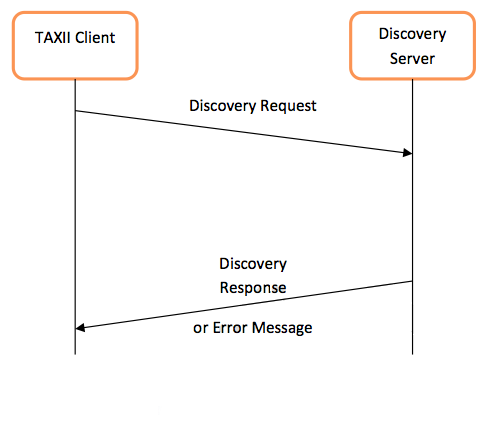
\includegraphics[width=150mm]{./Figures/DiscoveryExchange.png}
\end{figure}

El cliente TAXII envia un pedido de descubrimiento al servidor. Cuando el 
servidor recibe el pedido puede retornar un mensaje de error o pasar la 
información al Backend TAXII. Información relevante incluye la identidad 
autenticada si ésta fue provista. El Backend TAXII podría utilizar esta 
información junto a su propia política de control de acceso  para crear una 
lista de servicios a ser retornada. Esto podría ser empaquetado en una 
respuesta de discovery lo cuales podrían ser enviados al cliente TAXII. El 
cliente TAXII recibe esa respuesta y la pasa la información del servicio a su 
propio Back-End para ser procesado.

\subsection{Feed Information Exchange}

En este intercambio un cliente TAXII pide información sobre fuentes de datos disponibles en 
un Feed Server. El servidor responde con una lista de fuentes de datos 
disponibles. Dicha respuesta es realizada por back-end y se pueden considerar 
decisiones de control de acceso para realizar la respuesta.

\begin{figure}[ht!]
  \centering
    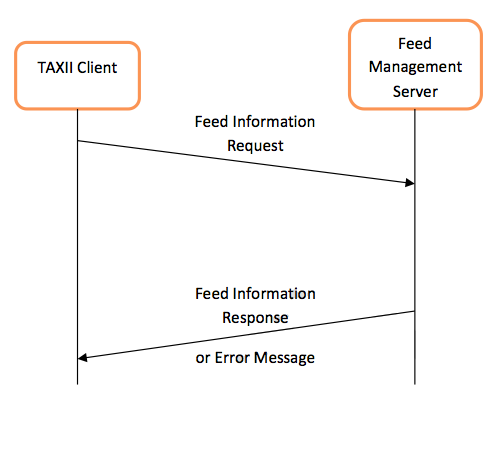
\includegraphics[width=150mm]{./Figures/FeedInformationExchange.png}
\end{figure}

En este intercambio, el cliente TAXII envia el Feed Information Request al 
servidor. Cuando el servidor recibe la request podría retornar un mensaje de 
error o pasar la información relevante al TAXII Back-end. Entre la información 
relevante se podría incluir la identidad. El Back-end podria utilizar esta 
información junto con sus políticas de control de acceso para crear una lista de 
fuentes de datos para ser enviadas al cliente. Esta lista es empaquetada en una 
Feed Information Response. El cliente recibe este mensaje y pasa el Feed a su 
propio Back-end para ser procesado.

\subsection{Subscription Managment Exchange}

En este un cliente intenta establecer, borrar, pausar, resumir o modificar una 
subscripción a un TAXII Data Feed conocido enviando un mensaje subscription 
managment request al servidor. El servidor pasa la request al TAXII Back-end el 
cual determina la respuesta. Esta respuesta es luego enviada al cliente.

\begin{figure}[ht!]
  \centering
    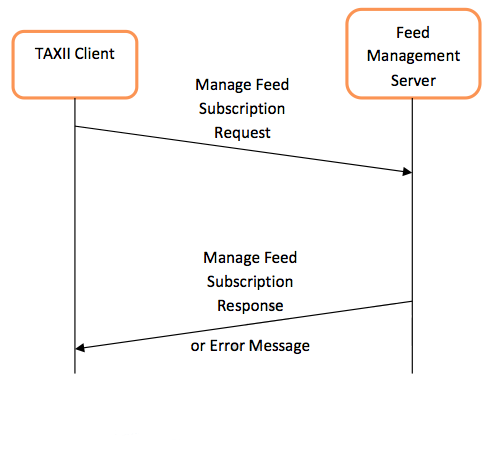
\includegraphics[width=150mm]{./Figures/SubscriptionManagmentExchange.png}
\end{figure}

El cliente TAXII envia una Manage Feed Subscription Request al servidor. Este 
podría retornar un mensaje de error TAXII o pasar la información relevante al 
TAXII Back-end. La información relevante podría incluir la identidad, parámetros 
que identifiquen la subscripción a ser modificada o creada, y la acción 
realizada. El Back-end TAXII puede usar dicha información junto con sus 
políticas de control de acceso y las funcionalidades que posea para determinar 
si la acción esta permitida o no. Dependiendo en la respuesta, el servidor 
podría retornar un mensaje de error TAXII o enviar una respuesta Manage Feed 
Successful Response.

\subsection{Feed Poll Exchange}

Es utilizado por un consumidor para pedir contenido de un productor de datos. El 
TAXII Data Feed content es enviado al consumidor en el mismo intercambio. Esto  
permite a un consumidor devolver el Data Feed Content en su propia tabla de 
tiempo y sin necesidad de utilizar un Inbox Server o aceptar conexiones 
entrantes.

\begin{figure}[ht!]
  \centering
    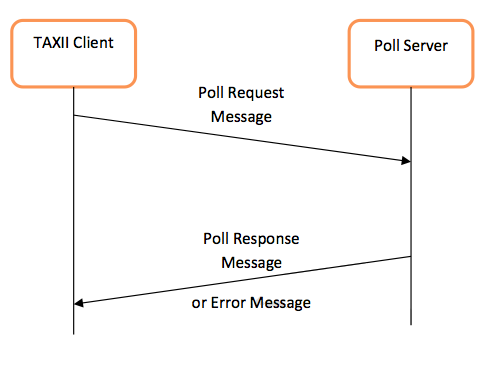
\includegraphics[width=150mm]{./Figures/FeedPollExchange.png}
\end{figure}

El cliente consumidor inicia el intercambio enviando un mensaje Poll Request al 
servidor de Poll del productor. El servidor puede enviar un mensaje de error 
inmediatamente o pasar la información relevante al TAXII Back-end. Información 
relevante incluye el nombre de la fuente, los parámetros de subscripción, 
timestamps indicando el intervalo de tiempo de la información que pide el 
consumidor y la identidad del consumidor. El back-end TAXII evalua esta 
información para determinar la respuesta. Hay tipos de respuesta posibles:
\begin{itemize}
  \item El pedido de información podria ser denegado. En este caso el servidor 
  de poll crea un error TAXII 
  \item Un conjunto de contenido TAXII Data Feed podria ser provisto. En este 
  caso , el servidor de Poll construira y enviara un mensaje de Poll Response. 
  Este mensaje indica el intervalo de tiempo que cubre el TAXII Data Feed que es 
  transmitido y los cuerpos de mensajes STIX que forman el contenido del TAXII 
  Data Feed.
\end{itemize}
En todos los casos, el cliente TAXII recibe el mensaje apropiado y pasa esta 
información al Back-end TAXII para ser procesado.

\section{Uso de TAXII}

Anteriormente se identifican distintos modelos utilizados por las comunidades para el 
el intercambio de información de amenazas informáticas. Estos modelos son 
Source/Suscriber, Peer-to-peer y Hub and Spoke. A continuación se  muestre como 
los servicios TAXII pueden ser utilizados para la implementación de dichos 
modelos.

\subsection{Source/Suscriber}

En este modelo una entidad es la fuente de información y algunos subscriptores 
tienen acuerdos con dicha entidad para recibir información periódicamente. Es 
deseado que los subscriptores no se conozcan entre si, para ello la fuente 
realiza acuerdos con cada uno de los subscriptores. En este modelo, la fuente es 
un productor TAXII mientras que los subscriptores son consumidores.

TAXII soporta este tipo modelo de intercambio con el uso de los servicios de 
Discovery, Feed Management, Inbox y Poll. Una organización que desee 
subscribirse al TAXII Data Feed de la fuente necesita conocer los servicios 
TAXII que la fuente ofrece y como contactar con ellos. Si bien esto podría ser 
realizado por una mecanismo fuera de banda (Publicar la información en otro medio)
también podría ser logrado contactando al servicio Discovery de la fuente. Desde 
este punto, el subscriptor podría contactar al servicio de Feed Managment 
identificado para aprender que fuentes ofrece el productor y que restricciones 
podría tener su acceso.

Si el contenido del TAXII Data Feed es restringido solo a algunas entidades 
autorizadas y el productor ha determinado que el subscriptor tiene permitido 
recibir el contenido, la fuente y el subscriptor necesitan acordar en como el 
subscriptor se autenticara. Dependiendo en el protocolo que soporta la fuente, 
esto se puede realizar por medio de una contraseña, un certificado o por otros 
medios. Si el contenido de un TAXII Data Feed es abierto y no requiere 
autenticación, este paso es innecesario cuando se establecen las subscripciones 
al TAXII Data Feed.

Una vez que la fuente es es capaz de autenticar al subscriptor (si es 
necesario), el subscriptor puede contactar al Feed Managment Service del 
productor y pedir subscripciones a las fuentes del productor. La fuente puede 
comparar dichos pedidos con su propio entendimiento de lo que el subscriptor 
puede recibir y permitir o denegar dichos pedidos según corresponda. La fuente 
puede enviar contenido al subscriptor al Inbox Service de este en el intervalo 
apropiado. Alternativamente, el subscriptor podría contactar al Poll service de 
la fuente para descargar el contenido deseado.

\begin{figure}[ht!]
  \centering
    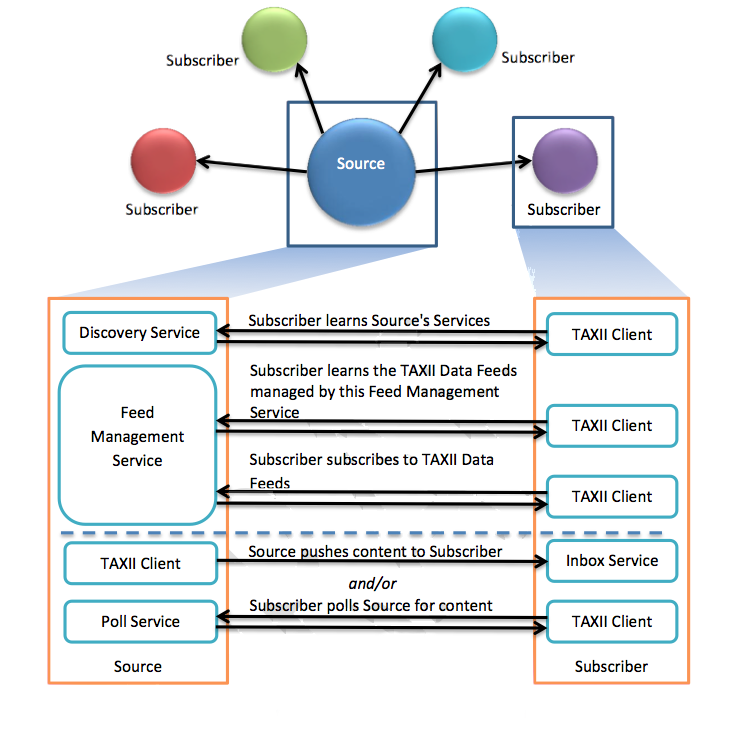
\includegraphics[width=150mm]{./Figures/SourceSuscriberModel.png}
\end{figure}

La figura mostrada como el modelo Source/Subscriber puede ser soportado por los 
servicios TAXII. El diagrama muestre los mensajes TAXII intercambiados entre la
fuente y el subscriptor. Con los intercambios que están por encima de la línea 
punteada se establece la subscripción. Los intercambios pueden ser realizados 
repetidamente sin la necesidad de realizar el proceso de subscripción 
nuevamente.

\subsection{Peer-to-peer}

En un modelo Peer-to-peer, los pares de organizaciones entran en un acuerdo 
mutuo para compartir su información entre ellos. En este modelo, cada Peer puede 
operar como productor y consumidor. Los socios en este intercambio podrían 
establecer fuentes utilizando un procedimiento similar al establecido en el 
modelo Source/Subscriber. Alternativamente, podrían acordar subir o descargar 
contenido sin ninguna subscripción formal. No tener una subscripción formal 
permitiria a un Peer albergar un Inbox Service sin necesidad de un Feed 
Managment Service.

El modelo Peer-to-Peer tiene dos variantes: acuerdos para el intercambio entre 
comunidades y acuerdos para el intercambio ad-hoc. En el primero la comunidad 
constituye acuerdos entre pares en los que todos los miembros acuerdan una única 
política la cual seguirán todos los miembros. A diferencia de los otros dos 
modelos que tienen un punto central desde el cual la información es diseminada, 
todo el intercambio ocurre de forma punto a punto entre los pares. Si dos pares 
cualquiera desean recibir información de otro directamente, estos necesitaran 
establecer un acuerdo apropiado con el otro para que el Peer le envíe 
información.

Alternativamente, el intercambio entre pares puede ser realizado de forma 
individual con intercambios ad-hoc. Esto podría ocurrir si dos compañías hacen 
acuerdos individuales para compartir entre ellas. En este caso, los acuerdos 
sobre que compartir son específicos para las partes. Una sola entidad podría 
participar en ambas variantes, perteneciendo a una o mas comunidades en las 
cuales los miembros comparten entre si siguiendo un acuerdo común entre los 
miembros y a su vez negocian acuerdos individuales con otras entidades. Alguna 
información recibida por medio de un acuerdo no siempre debería ser compartida 
con otros peers que no son parte del acuerdo. De esta forma un participante 
debería hacer un seguimiento de quien fue el proveedor de la información 
recibida, como se realiza ese seguimiento esta por fuera de la especificación de 
TAXII.

\begin{figure}[ht!]
  \centering
    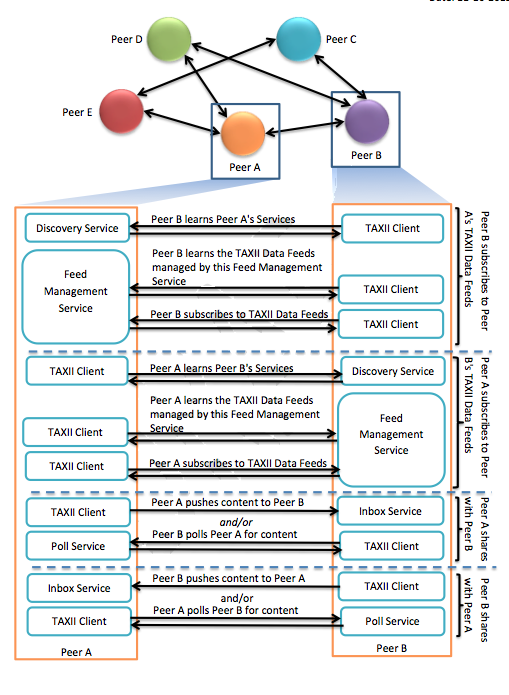
\includegraphics[width=150mm]{./Figures/PeerToPeerModel.png}
\end{figure}
\newpage
La figura anterior muestra como puede ser realizado el modelo Peer to peer por 
medio de los servicios TAXII. En este diagrama se ve que dos peers se contactan 
para pedir subscripciones para obtener información. Se asume que ambos peers 
tienen un Feed Managment Service que es utilizado para manejar todos los 
pedidos de subscripción.

\subsection{Hub and Spoke}

En un modelo Hub and Spoke, en este modelo la entidad Hub es un consumidor dede 
información que le proveen así como un productor que brinda información a un 
Spoke. Una entidad Spoke podría ser un productor, dando información al Hub, un 
consumidor que reciba actualizaciones del Hub o ambas. El Hub puede utilizar un 
Inbox Service para recibir información de cualquiera que desee enviar 
información de forma voluntaria y/o podría requerir información de ciertas 
fuentes para guardar la información en una única ubicación. Desde este punto, el 
Hub puede funcionar como una entidad Source del modelo Source/Subscriber 
mientras que los Spoke serían Subscribers de dicho modelo. El Hub puede adoptar 
cualquier política respecto de la información que recibe, desde pasar toda la 
información automáticamente a solo pasar información de socios reconocidos, o 
realizar ediciones y análisis antes de re enviar la información.

\begin{figure}[ht!]
  \centering
    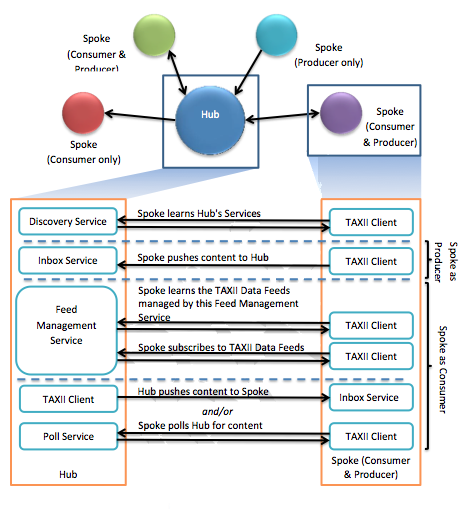
\includegraphics[width=150mm]{./Figures/HubAndSpokeModel.png}
\end{figure}
\newpage
La figura presentada muestra como se puede implementar el modelo Hub and Spoke 
utilizando los servicios provistos por TAXII. En este modelo algunas entidades 
Spoke podrían ser consumidores, otras productores y en algunos casos ambas. El 
diagrama muestra los intercambios que podrían ser utilizados por el Spoke que 
actúa como productor y consumidor. Si este desea actuar de una sola forma solo 
los intercambios necesarios serían relevantes. Independientemente del rol que 
tome el Spoke, es necesario que este conozca los servicios relevantes en el Hub. 
Esto se realiza utilizando el Discovery Service provisto por el Hub, de todas 
formas esto podría realizarse con mecanismos fuera de banda.

